\chapter{The Prevalence and Impact of Cheating in Online Multiplayer Games}

The integrity of online multiplayer games continues to be seriously compromised by the widespread use of cheats. This practice not only undermines fair play but also has a profound impact on player satisfaction and long-term engagement. In this chapter, we explore the extent of the cheating phenomenon, focusing particularly on \textit{Counter-Strike 2} (CS2), and argue that cheating constitutes one of the most significant threats to the sustainability of competitive online ecosystems. As the popularity of online titles grows, particularly those with competitive rankings and in-game economies, the incentives to cheat grow stronger, creating a persistent and evolving threat.

\section{Cheating as a Critical Threat to Player Retention}

Cheating is not a marginal problem—it is a critical factor driving user attrition. According to a global report by Irdeto, 60\% of players stated that cheating negatively impacted their multiplayer experiences \cite{irdeto2018global}. More alarmingly, 77\% of respondents indicated they would abandon a game if cheating persisted. These figures illustrate not only the widespread perception of unfairness but also the economic risk for developers, as high player churn can significantly affect active user metrics and revenue from in-game purchases.

\begin{table}[H]
\centering
\caption{Survey Results on Cheating in Online Games (Irdeto, 2018)}
\label{tab:irdeto-survey}
\begin{tabular}{|l|c|}
\hline
\textbf{Survey Statement} & \textbf{Percentage of Respondents} \\
\hline
Experienced negative impact due to cheating & 60\% \\
Would stop playing a game because of cheaters & 77\% \\
Support permanent bans for cheaters & 69\% \\
Believe developers are not doing enough & 55\% \\
\hline
\end{tabular}
\end{table}

These statistics highlight the severity of the problem: cheating not only degrades the moment-to-moment experience but also leads to long-term disengagement from the game. For games that rely on consistent engagement, particularly in esports ecosystems, this presents a fundamental challenge.

\section{Case Study: Cheating in \textit{Counter-Strike 2}}

\subsection{Player Base and VAC Ban Statistics}

\textit{Counter-Strike 2} remains one of the most popular online shooters. Notably, in February 2024, CS2 achieved a historic milestone with over 1.8 million concurrent players, surpassing previous records and reaffirming its dominant position within the competitive shooter genre. This growing player base intensifies the urgency to maintain integrity within the ecosystem, as the stakes for players, streamers, and the publisher rise proportionally.

However, this popularity comes with a cost: the game is plagued by a persistent community of cheaters. The Valve Anti-Cheat (VAC) system bans thousands of players each month, but the volume of bans illustrates the magnitude of the ongoing problem. Many cheaters use undetected private cheats or constantly create new accounts (smurfing), which reduces the long-term effectiveness of mass ban waves.

\begin{table}[H]
\centering
\caption{VAC Ban Statistics in CS2 (January--March 2025)}
\label{tab:vac-2025}
\begin{tabular}{|c|c|}
\hline
\textbf{Month} & \textbf{Number of VAC Bans} \\
\hline
January 2025   & 15,432 \\
February 2025 & 14,987 \\
March 2025   & 16,543 \\
\hline
\textbf{Total} & \textbf{46,962} \\
\hline
\end{tabular}
\end{table}

While these numbers reflect strong enforcement, they also suggest that the underlying problem remains unsolved. Many cheaters continue to bypass detection mechanisms, indicating that current anti-cheat technologies, though necessary, are insufficient. Additionally, the latency between cheat deployment and detection often allows cheaters to dominate matches for days or weeks before being banned.

\subsection{The Reporting System and Trust Factor Limitations}

CS2 incorporates a system known as the \textit{Trust Factor}, an invisible matchmaking metric introduced by Valve in late 2017 to improve the quality and fairness of online matches. Unlike traditional ranking systems, which focus primarily on in-game performance (e.g., win/loss ratio, kill/death ratio), the Trust Factor seeks to evaluate the overall behavior and reputation of a player across the Steam ecosystem.

Although Valve has not publicly disclosed the full algorithmic details of how Trust Factor is calculated, community research, developer hints, and user experimentation have led to the identification of several factors believed to influence the Trust Factor score:

\begin{itemize}
  \item \textbf{VAC bans and Overwatch bans:} Any history of cheating or toxic behavior significantly reduces Trust Factor.
  \item \textbf{Game-specific reports:} Frequency and validity of reports for cheating, griefing, or abusive conduct.
  \item \textbf{Commendations:} Positive in-game feedback from teammates (e.g., "Friendly", "Good Leader") is assumed to improve Trust Factor.
  \item \textbf{Steam account age:} Older accounts are generally considered more trustworthy than newly created ones.
  \item \textbf{Community participation:} Use of features like Steam Groups, Reviews, and profile visibility.
  \item \textbf{Hardware/software flags:} Suspicious configurations or third-party software may trigger internal risk indicators.
  \item \textbf{Behavior across multiple games:} Toxic behavior or bans in other Valve titles can influence Trust Factor globally.
  \item \textbf{Friend network quality:} Associations with banned or low-Trust players may negatively impact your own score.
\end{itemize}

Players with lower Trust Factor scores—often due to false reports, negative behavior, or even external factors—can find themselves matched with suspected cheaters or toxic teammates. The system does not communicate its internal logic to players, which contributes to confusion and a perception of arbitrariness.

Furthermore, the reporting system itself is vulnerable to abuse. Coordinated reporting by enemy players or even automated bots—known as \textit{report bots}—can unfairly penalize innocent users. These bots are sold as a service on underground forums and marketplaces, enabling malicious actors to artificially lower another player's Trust Factor through mass false reports. Victims of such actions may find themselves trapped in low-quality matchmaking pools with increased exposure to cheaters.

Conversely, a market has emerged for \textit{commend bots}, which artificially inflate Trust Factor scores by using botted accounts to issue in-game commendations. These commendations, such as "Good Leader", "Friendly", or "Teacher", are believed to be positively weighted in Trust Factor calculations. These services exploit the opacity of Trust Factor metrics and undermine the intended spirit of fair matchmaking by allowing players to manipulate their standing through paid influence.

Consequently, while the Trust Factor system aims to protect competitive integrity, its opacity and susceptibility to manipulation can exacerbate the issues it was designed to mitigate. Calls for greater transparency, audit trails, and player-facing Trust metrics have been common within the community, especially among long-term and high-investment users.

\subsection{Economic and Psychological Impact}

Valve's ban waves have economic repercussions as well. In early 2025, a VAC wave eliminated accounts with over two million USD in inventory value \cite{ggscore2025vacban}. This not only disrupted the secondary skin market but also created anxiety among legitimate players. Many users invest both time and money into building inventories, and the fear of false positives or lack of transparency in ban decisions can alienate loyal players.

The psychological burden is also considerable: legitimate users who are falsely flagged or who perceive the system as ineffective may lose confidence in the platform, resulting in churn. In ranked systems, where competition is meant to be meritocratic, repeated exposure to cheating can erode motivation and participation. For new players, early exposure to blatant unfairness can lead to immediate disengagement.

Moreover, the persistent presence of cheaters devalues competitive ranks and tournaments, potentially deterring sponsors and professional teams from engaging with the title long-term. In such an environment, even minor perceived imbalance can be seen as systemic failure, amplifying negative sentiment across the community.

\section{Community Perception and Player Sentiment}

The response from the gaming community is often one of frustration, skepticism, and fatigue. On platforms like Reddit, Steam, and YouTube, countless posts and videos chronicle blatant cheaters in ranked games, sometimes persisting for weeks without enforcement. These examples accumulate into a narrative of neglect, regardless of the actual efforts made by developers.

Professional players and streamers have also spoken out, emphasizing how recurring cheating incidents damage both their gameplay experience and viewer engagement. For example, repeated matches against obvious cheaters during live broadcasts diminish entertainment value and create reputational risks for the publisher.

This perception of systemic vulnerability further undermines confidence in anti-cheat frameworks and leads to a normalization of defeatism among legitimate players. Forums often reflect sentiments such as "everyone is cheating at higher ranks" or "VAC does nothing," which signal the erosion of perceived fairness.

In a competitive environment where rank integrity is paramount, even a minority of cheaters can poison the perception of fairness. This phenomenon fuels resignation and, eventually, player abandonment. A toxic perception climate can spread faster than actual cheating prevalence, compounding the damage.

\section{Legal and Ethical Implications of Cheating Software}

Beyond technical responses, several companies have turned to legal action. The production and distribution of cheat software violates terms of service and, in some jurisdictions, constitutes intellectual property infringement or even fraud.

Bungie and Ubisoft, for example, have successfully sued cheat developers for their role in undermining game integrity and profiting from illicit tools. Notably, in 2023, Bungie won a \$12 million lawsuit against cheat seller AimJunkies for its role in distributing software that compromised \textit{Destiny 2}'s ecosystem. Other cases have followed in Australia, Germany, and the United States, with courts increasingly recognizing the damages associated with commercial cheating operations.

These legal precedents are critical not only for deterrence but also to assert the enforceability of end-user license agreements (EULAs) in gaming contexts. They signal that companies are increasingly willing to pursue judicial avenues when technical means fall short. Legal actions also help target the source of advanced cheat development, limiting their distribution and profitability.

From an ethical perspective, the existence of pay-to-win cheats challenges the spirit of competitive gaming. When fairness is monetized and subverted, the entire premise of esports and ranked systems is put into question, leading to long-term damage to brand value and consumer trust.

\section{Anti-Cheat Technologies and Their Limitations}

While developers continue to enhance their anti-cheat frameworks, existing solutions often operate reactively. Valve’s VAC system relies on detecting known cheat signatures. Although the update to VacNet 3.0 brings improvements in behavioral analysis and detection latency \cite{vacnet2025update}, many cheats remain undetected due to obfuscation, polymorphism, and manual injection methods.

Furthermore, VAC does not operate at the kernel level, leaving a gap exploited by more sophisticated cheating tools. Unlike Riot’s Vanguard, which implements invasive low-level monitoring, VAC opts for user privacy—but at the cost of reduced enforcement power. This trade-off reflects a broader industry dilemma between effectiveness and user rights.

More innovative systems, such as AI-driven cheat behavior modeling or client-side encryption, are being tested, but none have yet offered a comprehensive solution. Cheat developers adapt quickly, often using anti-debugging and virtualization evasion techniques, requiring anti-cheat providers to continually evolve in a costly and time-sensitive arms race.


Cheating poses a systemic threat to the health and sustainability of online multiplayer games. The data reveals that while anti-cheat systems like VAC are essential, they are not enough to eliminate the problem. The high number of bans, combined with persistent community frustration and the economic damage inflicted, indicate that many cheaters continue to escape detection.

To restore trust and ensure fair play, the industry must explore more proactive, transparent, and adaptive anti-cheat solutions, supported by legal frameworks and community-driven oversight. Educational initiatives, transparency reports, real-time user flagging tools, and tighter platform-level enforcement (e.g., via Steam or Xbox Live) could help close current enforcement gaps. Without such evolution, even the most successful titles risk losing their competitive legitimacy and alienating their player base.





\begin{figure}[H]
    \centering
    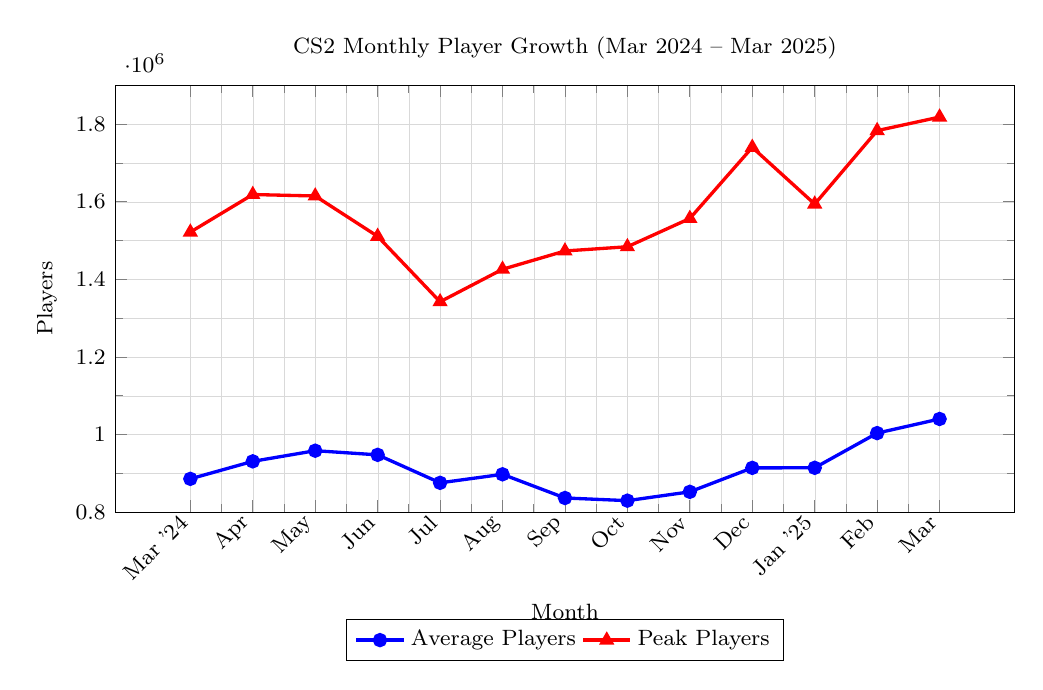
\begin{tikzpicture}
      \begin{axis}[
        width=13cm,
        height=7cm,
        xtick=data,
        xticklabels={
          Mar '24, Apr, May, Jun, Jul, Aug,
          Sep, Oct, Nov, Dec, Jan '25, Feb, Mar
        },
        xticklabel style={rotate=45, anchor=east, font=\footnotesize},
        yticklabel style={font=\footnotesize},
        xlabel=Month,
        ylabel=Players,
        xlabel style={font=\footnotesize},
        ylabel style={font=\footnotesize},
        title={\footnotesize CS2 Monthly Player Growth (Mar 2024 – Mar 2025)},
        legend style={
          font=\footnotesize,
          at={(0.5,-0.25)},
          anchor=north,
          legend columns=2
        },
        grid=both,
        grid style={line width=.1pt, draw=gray!30},
        minor tick num=1,
        tick style={line width=0.3pt},
        every axis plot/.style={very thick},
        ymin=800000, ymax=1900000,
      ]
    
      % Average Players
      \addplot[blue, mark=*] coordinates {
        (0,885629.7) (1,930749.0) (2,958207.3) (3,947520.5) (4,875365.1) (5,897337.9)
        (6,836306.7) (7,829438.8) (8,852164.3) (9,913953.4) (10,914092.2) (11,1003570.6) (12,1040008.9)
      };
      \addlegendentry{Average Players}
    
      % Peak Players
      \addplot[red, mark=triangle*] coordinates {
        (0,1521796) (1,1618685) (2,1614925) (3,1510840) (4,1342171) (5,1425958)
        (6,1473144) (7,1484045) (8,1556938) (9,1740261) (10,1594016) (11,1783434) (12,1818368)
      };
      \addlegendentry{Peak Players}
    
      \end{axis}
    \end{tikzpicture}
    \caption{\footnotesize Counter-Strike 2 player count evolution over the past 13 months.}
    \label{fig:cs2-growth}
    \end{figure}
    